\chapter{TLS echoservice}

The web services which were presented in the previous chapters have one mayor drawback: the communication between the two endpoints is unsecure.
Due to that reason the current and the next chapter will discuss how to create a secure web service.
In general security in a network can be subdivided into the following categories:~\cite{TANNENBAUM_2001}\task{verfiy citation}
\begin{itemize}
	\item \textbf{Confidentiality} --- Protection of the data against passiv attacks (such as publicise message content)
	
	\item \textbf{Authentication} --- Verification of the Authenticity  of the communications partner.

	\item \textbf{Integrity} --- Protection against interception and manipulation,replay,insertion, etc.  of a message.

	\item \textbf{Non-repudiation} --- Preventing the sender to repudiate the message transmitted by him.

	\item \textbf{Access control} --- Restrict the access to ressources.

	\item \textbf{Availability} --- Ensure a system is always usable which is challenged by several attacks.

\end{itemize}
%1-21   Gebräuchliche Dienste
%     Identifizierung           Vermerk
%     Berechtigung              Zugriff
%     Lizenz/Zertifizierung     Gültigkeitsprüfung
%     Unterschrift              Zeitpunkt des Auftretens
%     Bezeugung                 Abstimmung
%     Übereinstimmung           Eigentum
%     Zuverlässigkeit           Registrierung
%     Quittungen                Genehmigung/Verbot
%     Bestätigung des Ursprungs Privatsphäre
%
% Nach Sicherheit in verteilten Systemen, ITM Lübeck
Ideally all six categories should have been achieved by such an application (though the last category, availability, is difficult to realise).
In the present chapter, the security will be put into practice by extending the protocol stack with an additional security layer called TLS (Transport Layer Security). Due to the location after the TCP and the HTTP layer, the layer is only capable to limitate the access to the grid to a certain set of users.
Nevertheless it provides the security categories: Confidentiality, authentication, integrity, non-repudiation and access control.\\


In the next section gives a basic understanding of the working principale of the TLS. Emphasis is put on the security concept and not on an exact description of the technical realisation in order to enable newcomers an entry to  this area.


% It is recommand to satifiy as much categories as possible. 
%authentication , confidentiality and integrity protection of TCP-based communication --- non-repudiation due to private key, access control to our service.


\section{Transport Layer Security}


The TLS is a protocol which provides a secure connection between two endpoints. It is located directly upon the TCP/IP layers and uses typically an asymmetric encryption to establish the connection (alternatively a symmetric pre-shared key may be used). After the communication has successfully established, both participants are switching to another encryption method which is based on a new negotiated symmetric key.\\
%    1. Peer negotiation for algorithm support
%    2. Key exchange and authentication
%    3. Symmetric cipher encryption and message authentication   - from wikipedia
%
%


Symmetric and asymmetric encryption are the two main classes of cryptography algorithms.
In case of a symmetric encryption both participants are holding the same secret key. 
Symmetric encryption can be ranked as being very secure but its downside is that the key distribution is very difficult in practice.
The key has to be shared previously, ideally over a secure channel which is may either be a complete diffrent medium (i.e. a letter, speech) or a channel which has been encrypted with another secret key.
Asymmetric encryption follows a diffrent functional principle. While the symmetric encryption utilise one shared secret, the asymmetric ecryption is based on two keys: a private key and public key. As the names imply the private key is kept secret and is never shared while the public key is available to everyone. Messages encrypted with the public key can only be decrypted with the private key and the other way round, messages encrypted with the private key can only be decrypted with the public key. The Figure~\ref{fig:asymmetric_encryption} illustrates the circumstances of the case.\\
\begin{figure}[htb]
	\centering%epstopdf async.eps
	\subfloat[Texttext\label{fig:cgd}]
		{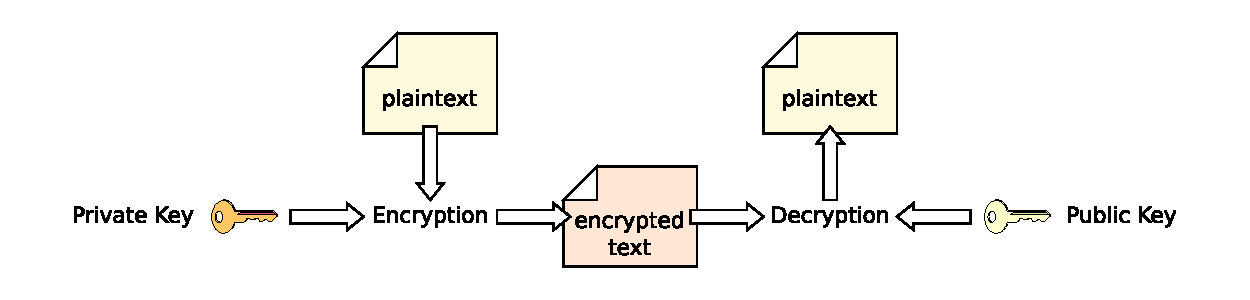
\includegraphics[width=12cm]{tex_tls_echoservice/async.pdf}}\\
	\subfloat[Texttext\label{fig:cgd}]
		{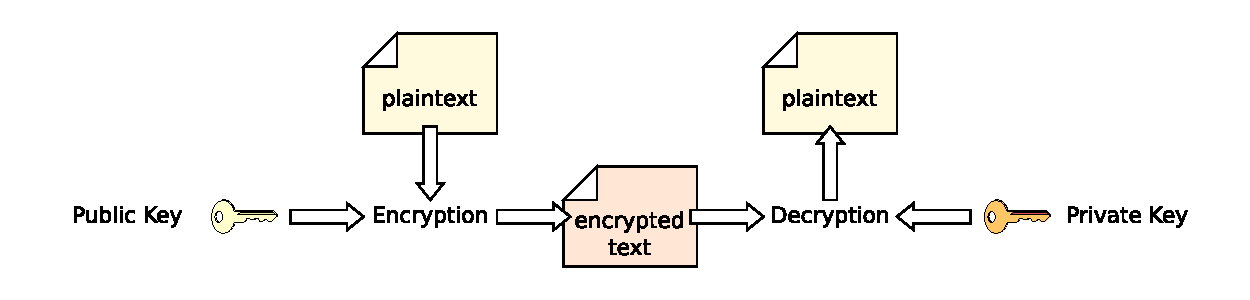
\includegraphics[width=12cm]{tex_tls_echoservice/async2.pdf}}
	\label{fig:asymmetric_encryption}
	\mycaption{specific}{general}
\end{figure}


At startup of the communication process A (Alice) who desires a secure connection transmits her public key to B (Bob).
Bob is now able to encrypt the messages such that only A is able to decrypt them.
As one can see this first approach already provides confidentiality and integrity of messages.
%
Non-repudiation, authentication and due to that access control are not given because the identity of Alice is not proven.
In order to be able to check identities so called certificates must be introduced.
Certificates render the possibility to validate the identity of its owner. They are signed by a certificate authority (CA) which's identity can be resolved to another CA or which is  pre-configured to be trusted.
A certificate is composed of its owner's public key, his identity, the name of the signing CA and a signiture which is a hash-value of the certificate encrypted with the private key of the CA. 
If a certificate can be resolved to a CA with is pre-configured to be trusted, the identity of the certificate owner is considered as to be proven. 
In general a set of trusted CAs is already defined in the operation system.
To obtain a certificate a certificate request has to be submitted to a CA.
After the CA has verified the identity of the requesting person and the requested certificate will be signed.
Figure~\ref{fig:certificate_request} shows the procedure of gaining a certificate.
\begin{figure}[htb]
	\centering%epstopdf certificates.eps
 	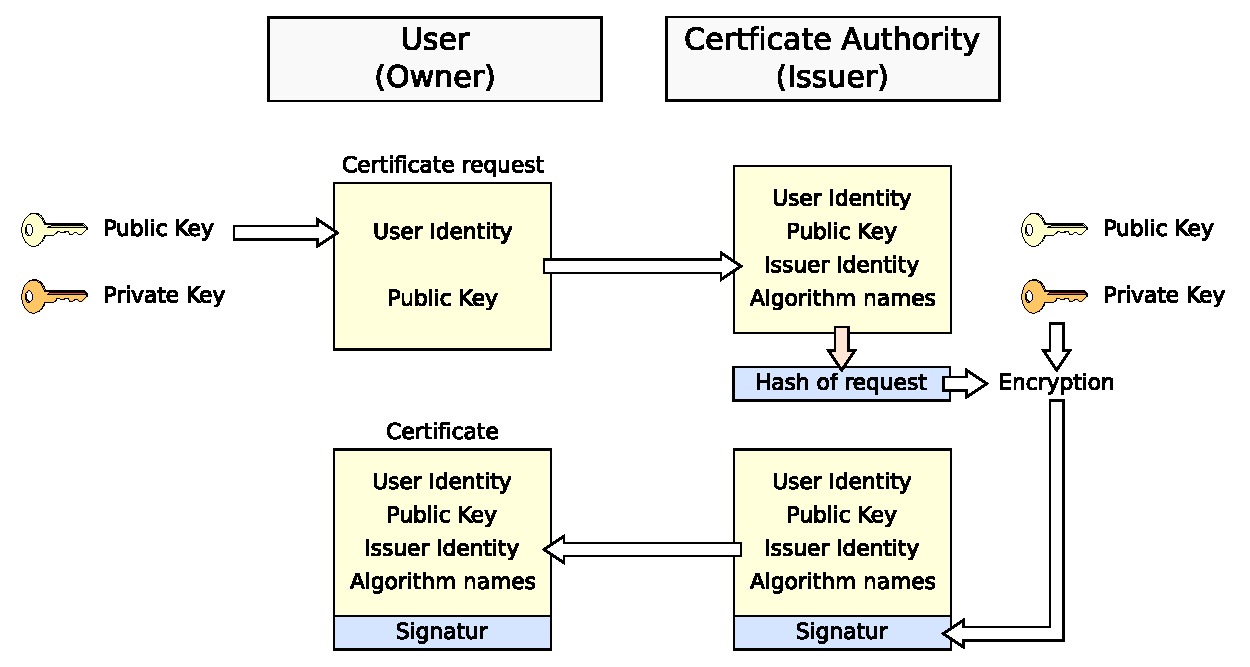
\includegraphics[width=13cm]{tex_tls_echoservice/certificates.pdf}
	\mycaption{specific}{general}
	\label{fig:certificate_request}
\end{figure}
In the first step, a private and a public key will be generated by the requester. The public key together with a textual description of the identity  depict the request which will be transmitted to a CA. After the CA successfully varified the validity of the request, the identity of the CA and the name of used the encryption algorithms are added.
The collected data will represent the plain text of the certificate. In order to ensure the integrity of the text, 
a hash value will be created. (A fixed-sized short string which is generated by an algorithm based on an arbitrary long given text. The algorithm is designed such that a small change in the text will cause the hash value to change almost like a random function. Thus, the hash value can be used a fingerprint of the text.) The CA signs the plain certificate by encrypting its hash value with its private key. Finally the signed certifcate will be returned to the requester.
%
%
If an outside person wants to verify the certificate owner, the encrypted hash value has to be decrypted by the public key of the CA and a hash value has to be created with the same algorithm in order to compare them.\\


Figure~\ref{fig:verification_of_certificates} shows a usecase in which Alice wants to resolve the identity of Bob. Alice submitts her request to Bob along with a challange consisting of a random number $n$. 
The random number ensures that it is not possible to repeat a message (integrity).
Bob encrypts the number with his private key and returns it together with his certificate. Alice uses the public key of Bob to decrypt the challange. 
If the decrypted number is equal to the transmitted number, Alice can reason that the identity of Bob is to be trusted in case she is trusting the CA which has signed Bobs certificate. 
%
In the given example Alice only trusts the CA 2 but not CA 1.
In order to resolve the identity, Alice establishes a connection to CA 1 and submits another random number $n$ as a challenge.
The CA 1 encrypts the challange with its private key and send the result along with its certificate back to Alice. Alice succefully validates the certificate of CA 1. Due to the certificate was signed by CA 2 which is pre-configured to be trusted she can follow to trust CA 1 and in conclusion the identity of B. In summary, Alice knows she is talking to Bob. If Bob also wants to be sure how he's talking to the same procedure has to be done for the identity of Alice. The TLS mode in in which both endpoints are ensuring themself to whom they are talking to is called bilateral connection.
Due to the client is aware of the service authentity, the confidential treatment of his data is given such that it won't be revealed to a third party (service sided confidentiality). Moreover the access to the service can be controled (access control) and the results are only passed back to the right person (client sided confidentiality). 
As one can see confidentiality, authentication, integrity and non-repudiation are now given.\\
\begin{figure}[htb]
	\centering%epstopdf verification.eps 
	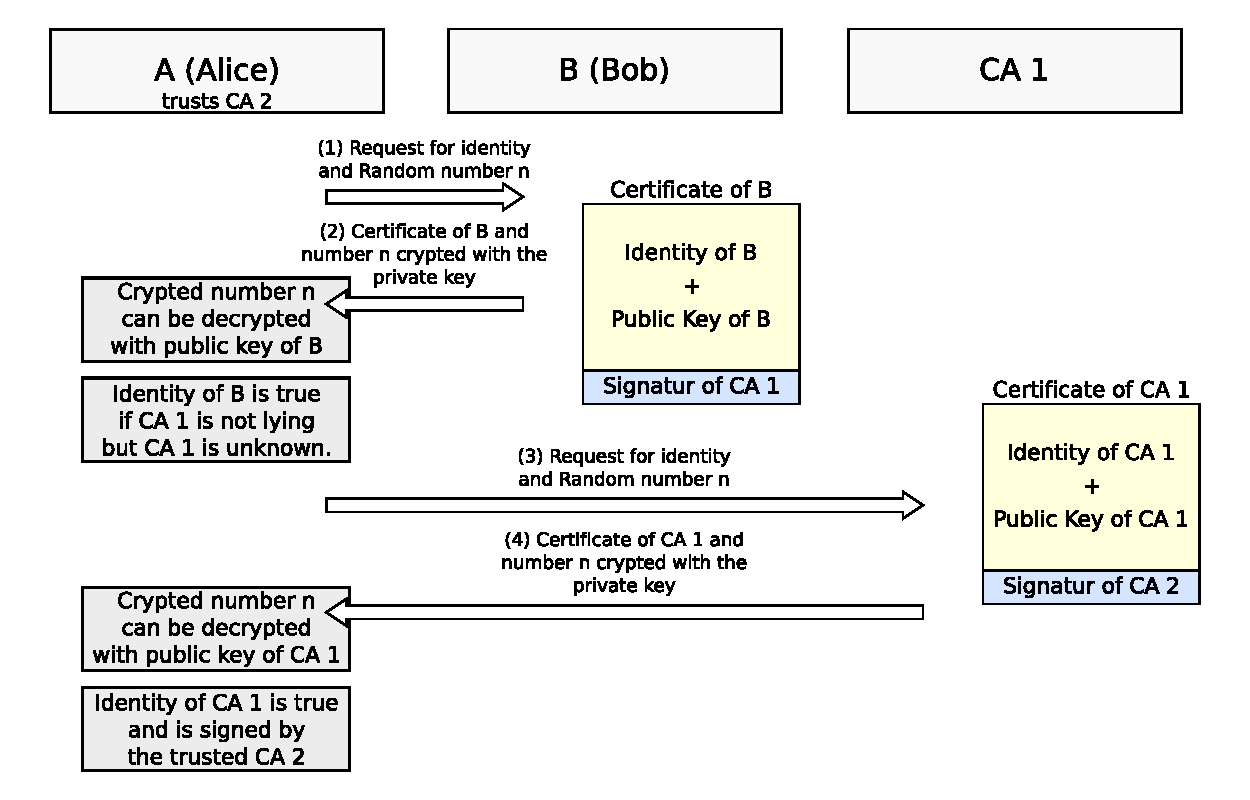
\includegraphics[width=13cm]{tex_tls_echoservice/verification.pdf}
	\mycaption{specific}{general}
	\label{fig:verification_of_certificates}
\end{figure}



Certificates have several advantages. They are scaling very good with the amount of users because CAs can create new sub-CAs such that the load is balanced (certificates of a CA may be cached). Furthermore no critical information is exchanged which may gets intercepted - in particular no secret key is shared. Instead a set of pre-configured CAs which will be in general provided by the operation system is needed.
In respect of ARC it is obvious, that the access to the grid should be under control of its administrator. To do so, the administrator have to build up his own CA to be in charge of creating certificates for a set of users. 
The created CA have to be shipped into the directory of pre-configured CAs.
(Within the source code there are two shell scripts to create a CA and related certificates). Due to there's a bunch of tools for certificates (like \textit{openssl}) it is easy to maintain them. 


o Infrastructure is given and easily to maintain

o In general the pre-configured organistion take money to sign certifcates, but they can also be created locally.

o VOMs are realisable

ARC:

TLS also supports the more secure bilateral connection mode (typically used in enterprise applications), in which both ends of the "conversation" can be ensured with whom they are communicating




o What do we need to get a service running

clientCA   - Authority guarantee for identity
clientCERT - Certificate given
clientKEY  - Secret key of the client to read messages, encrypted by the public key in the certificate!

serverCA   - Authority guarantee for cert. CA is known by the server. If not, the encrypted cert can be read be its CA.
serverCERT - Certificate given by the CA. Contains a snippet which can be read by the Public key of the CA.
serverKEY  - Secret key of the client to read messages, encrypted by the public key in the certificate!


Server has got have:
Its  serverCERT serverKEY and some kind of root CA knowing the client
Client has got to have
Its  clientCERT clientKEY and some kind of root CA knowing the server



\task{RENAMING into~ARC service configuration file}
\task{echo service client configuration file}






%The first two goals can be reached by encrypting the channel/connection between client and server. An approach 
%sich bewähren / behaupten
%which stand the test of time is to introduce a TLS (Transport Layer Security) also known as SSL (Secure Sockets Layer).
%Authenticity, Confidentiality, Integrity
%The client wants to reassure himself to send his vulnerable data only to the server who can prove its correct identity.
%Furthermore a prove of authenticity is needed. % Sich versichern, dass das Gegenüber der ist, für welchen er sich ausgibt
%It .... does fancy stuff ...
%
%
%Authorization:  The server on the other side takes an interest in limitate its ressources to a close circle of users. Above all no %foreign clients shall be able to use the services.\\


\clearpage
\section{Service}

One can add the TLS in client and server by simply extending the arched configuration file and a small modification of the client.



WARNING: If the programm fails, check if one of your certifacte is expired. If so, create new one using the script files in the directory 'certFactory'

For HED is build up to  % entsrprechend einer Mod Structur
be modular, the security can easily be extend to our given example.
Each Message Chain Component (MCC) or service has a common interface for implementing various pluggable components (plug-ins) called SecHandler. The SecHandler components provide a method for processing messages traveling through Message Chains of the HED. 
Each MCC or Service usually implement two queues of SecHandlers – one for incoming messages and one for outgoing called “incoming” and “outgoing” respectively. All SecHandler components attached to the queue are executed sequentially. 
If any of them fails, message processing fails as well. 
Each SecHandler is configured inside the arched configuration file used for configuring whole chain of MCCs 
Some of the currently implemented SecHandler components make use of pluggable and configurable sub-modules called Policy Decision Point (PDP). PDP can process ARC specific Request and Policy documents which are as well written in XML format~\cite{QIANG_2008}..




4 types:
                <KeyPath>./clientKey.pem</KeyPath>
                <CertificatePath>./clientCert.pem</CertificatePath>
                <CACertificatePath>./serviceCA.pem</CACertificatePath>

\lstsetCPP
\lstinputlisting
	[
	label=lst:tls_echo_service_cpp,
	caption={[HED configuration file for the Arc intern echo service. Filename: arcecho\_no\_ssl.xml]
	\textbf{HED configuration file for the Arc intern echo service. Filename: arcecho\_no\_ssl.xml\textcolor{white}{hmf}}}
	]
{../src/services/tlsechoservice/tlsechoservice.cpp}




\lstsetARCHEDXML
\lstinputlisting
	[
	label=lst:tls_echo_arched_xml,float=htb,
	caption={[HED configuration file for the Arc intern echo service. Filename: arcecho\_no\_ssl.xml]
	\textbf{HED configuration file for the Arc intern echo service. Filename: arcecho\_no\_ssl.xml\textcolor{white}{hmf}}}
	]
{../src/services/tlsechoservice/arched_tls_echoservice.xml}


\lstsetKSH
\begin{lstlisting}[
label=lst:tls_echo_arched_invoke,float=htb,
caption={[Transformation in eine uniforme konzentrische Verteilung.]
         \textbf{Transformation in eine uniforme konzentrische Verteilung.\textcolor{white}{hmf}}}]
$ rm -f /var/log/arched.log
$ arched -c arched_echoservice.xml  && echo jo ||echo n
$ tail -n100 -f /var/log/arched.log
$ killall arched
\end{lstlisting}




\clearpage
\section{Client}

\lstsetCPP
\lstinputlisting
	[
	label=lst:tls_echo_client_cpp,
	caption={[HEC configuration file]
	\textbf{HEC configuration file\textcolor{white}{hmf}}}
	]
{../src/clients/tlsechoclient/tlsechoclient.cpp}



Folgender XML Aufruf und Antwort soll \textit{automatisch} generiert werden:

%[caption={[]WegDamit},language=XML,basicstyle=\scriptsize,breaklines=true,label=lst:request] 





Zertifikate
Zustände (Nutzer wiedererkennen, arbeit aufnehmen)




\lstsetKSH
\begin{lstlisting}[
label=lst:tls_echo_client_invoke,float=htb,
caption={[Transformation in eine uniforme konzentrische Verteilung.]
         \textbf{Transformation in eine uniforme konzentrische Verteilung.\textcolor{white}{hmf}}}]
$ ./echoclient
Tue Feb 17 17:04:08 2009
\end{lstlisting}






\lstsetJUSTXML
\begin{lstlisting}[
label=lst:tls_echo_request_XML,float=htb,
caption={[Transformation in eine uniforme konzentrische Verteilung.]
         \textbf{Transformation in eine uniforme konzentrische Verteilung.\textcolor{white}{hmf}}}]
<soap-env:Envelope xmlns:tlsecho="urn:tlsecho" xmlns:soap-enc="http://schemas.xmlsoap.org/soap/encoding/" xmlns:soap-env="http://schemas.xmlsoap.org/soap/envelope/" xmlns:xsd="http://www.w3.org/2001/XMLSchema" xmlns:xsi="http://www.w3.org/2001/XMLSchema-instance">
  <soap-env:Body>
    <tlsecho:tlsechoRequest>
      <tlsecho:say operation="ordinary">text_to_be_transmitted</tlsecho:say>
    </tlsecho:tlsechoRequest>
  </soap-env:Body>
</soap-env:Envelope>
\end{lstlisting}






\lstsetJUSTXML
\begin{lstlisting}[
label=lst:tls_echo_response_XML,float=htb,
caption={[Transformation in eine uniforme konzentrische Verteilung.]
         \textbf{Transformation in eine uniforme konzentrische Verteilung.\textcolor{white}{hmf}}}]
<soap-env:Envelope xmlns:tlsecho="urn:tlsecho" xmlns:soap-enc="http://schemas.xmlsoap.org/soap/encoding/" xmlns:soap-env="http://schemas.xmlsoap.org/soap/envelope/" xmlns:xsd="http://www.w3.org/2001/XMLSchema" xmlns:xsi="http://www.w3.org/2001/XMLSchema-instance">
  <soap-env:Body>
    <tlsecho:tlsechoResponse>
      <tlsecho:hear>[ text_to_be_transmitted ]</tlsecho:hear>
    </tlsecho:tlsechoResponse>
  </soap-env:Body>
</soap-env:Envelope>
\end{lstlisting}

